\paragraph{Ricerca}

\subparagraph{Ricerca}

\label{Ricerca}

\begin{figure}[ht]
	\centering
	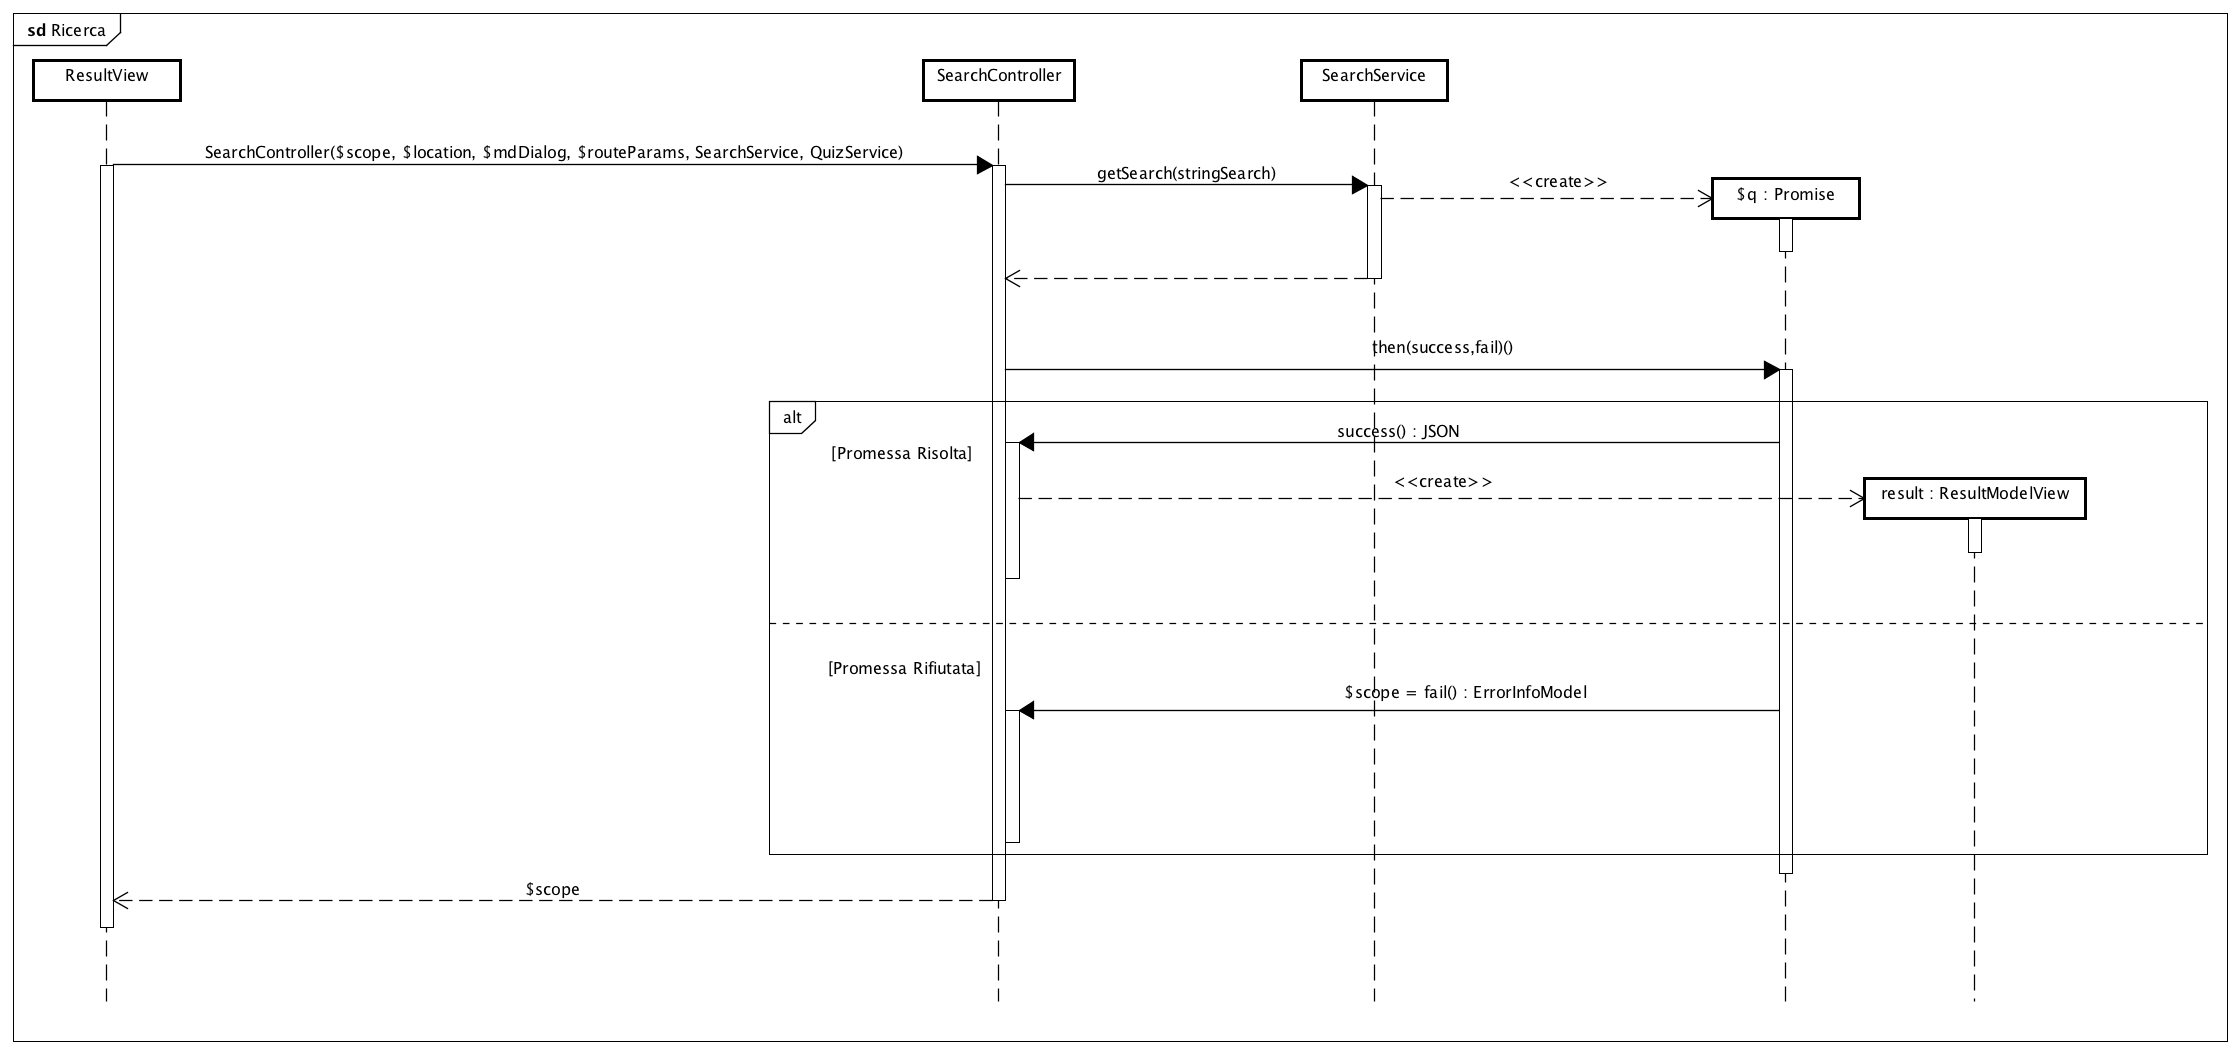
\includegraphics[scale=0.260,keepaspectratio]{UML/DiagrammiDiSequenza/Front-end/Search.png}
	\caption{Ricerca}
\end{figure} \FloatBarrier

L'utente, dopo aver effettuato una ricerca, viene indirizzato alla pagina di ricerca. Una volta posizionato in questa pagina, \textit{Angular\ped{G}} provvederà a costruire la classe \texttt{SearchController}. Durante la creazione di tale classe viene eseguita la ricerca mediante \texttt{SearchService}. Questo \texttt{service\ped{G}} restituisce una promessa, se questa verrà rispettata verrà popolato l'attributo \texttt{result} altrimenti verrà restituito un oggetto di tipo \texttt{ErrorInfoModel} e mostrato a video mediante \texttt{\$mdDialog}.

\subparagraph{Iscrizione ad un questionario}

\label{Iscrizione ad un questionario}

\begin{figure}[ht]
	\centering
	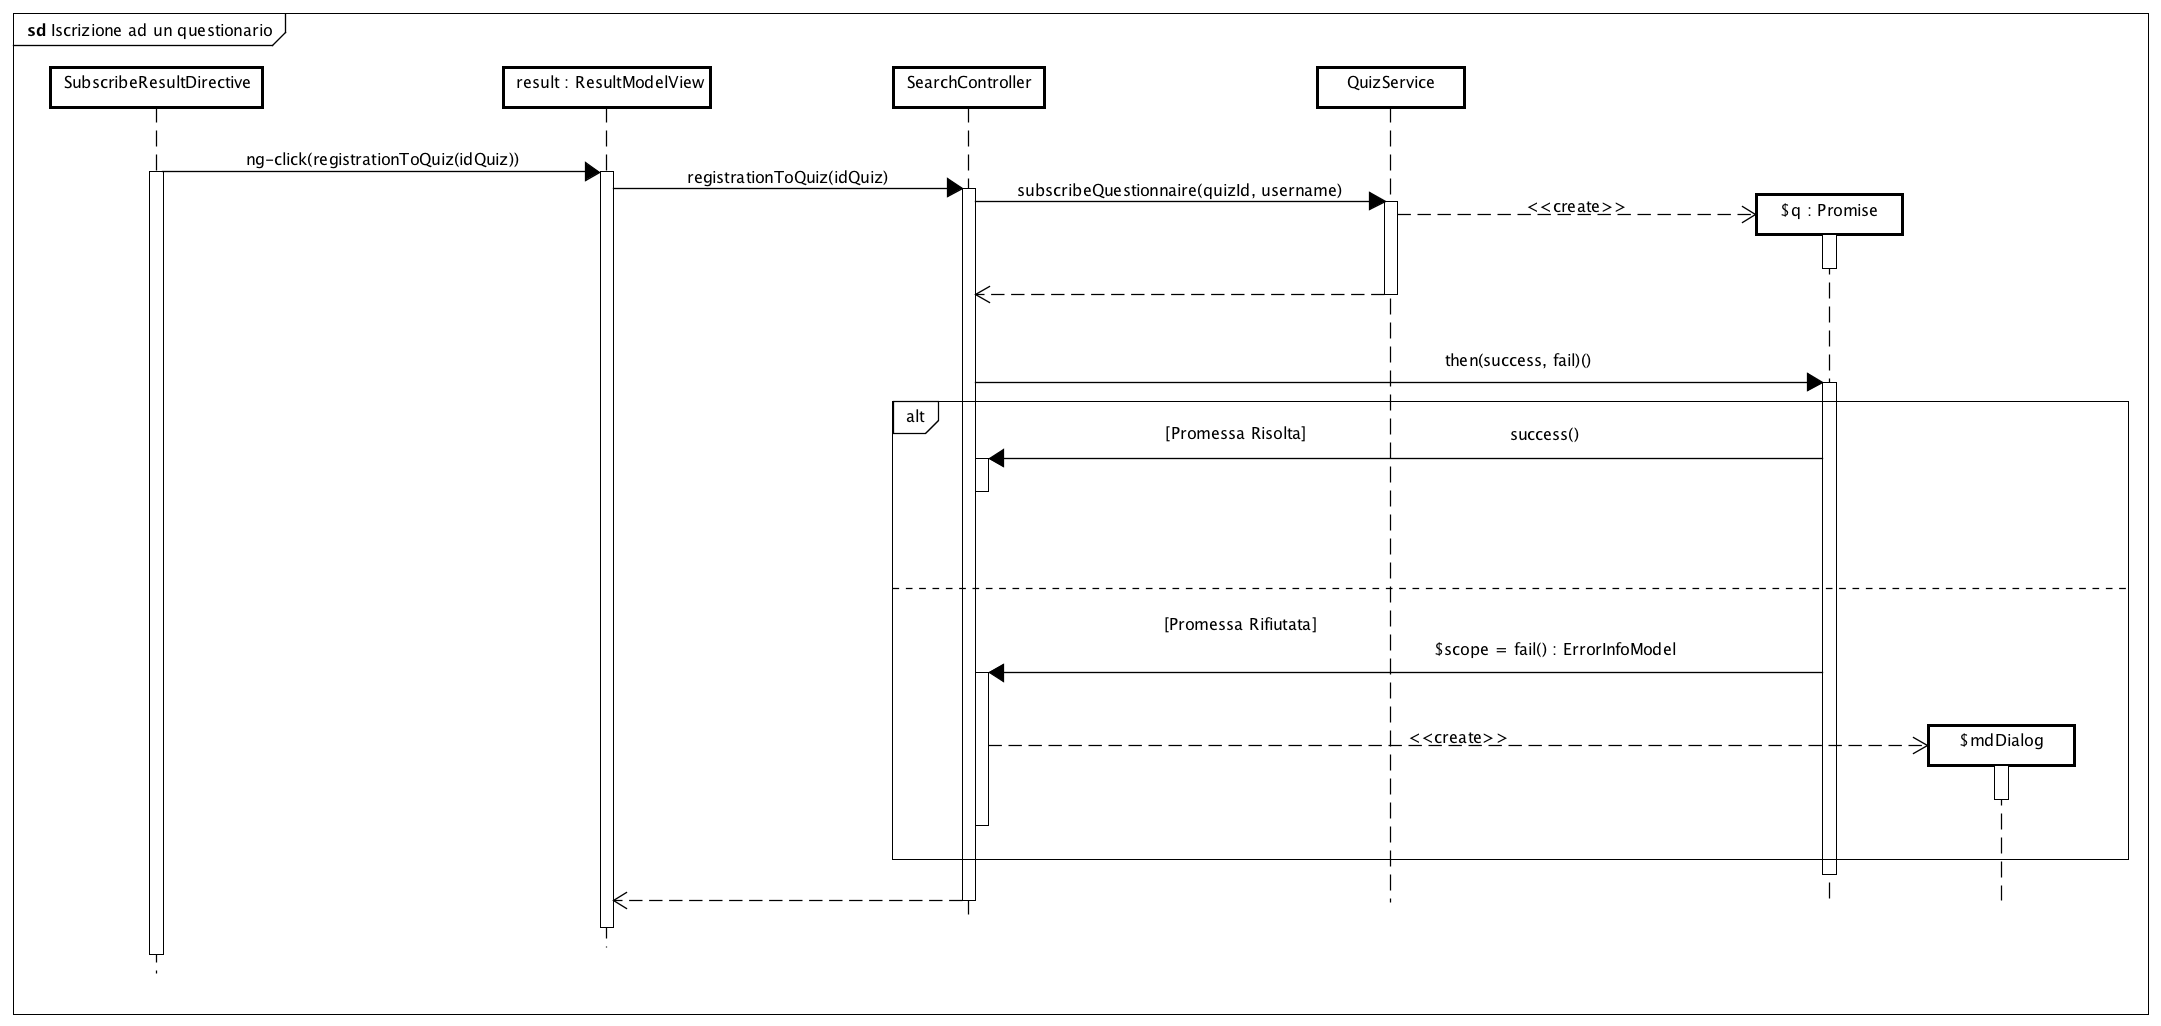
\includegraphics[scale=0.275,keepaspectratio]{UML/DiagrammiDiSequenza/Front-end/Search_subscribeToQuiz.png}
	\caption{Iscrizione ad un questionario}
\end{figure} \FloatBarrier

L'utente, posizionato dentro la pagina di ricerca, potrà iscriversi ad un questionario azionando l'evento associato al bottone di iscrizione al questionario. Attraverso \texttt{SearchController} viene eseguita l'iscrizione mediante \texttt{QuizService}. Questo \texttt{service\ped{G}} restituisce una promessa, se accadrà un errore verrà restituito un oggetto di tipo \texttt{ErrorInfoModel} e mostrato a video mediante \texttt{\$mdDialog}.


\subparagraph{Redirect alla pagina di un utente}

\label{Redirect alla pagina di un utente}

\begin{figure}[ht]
	\centering
	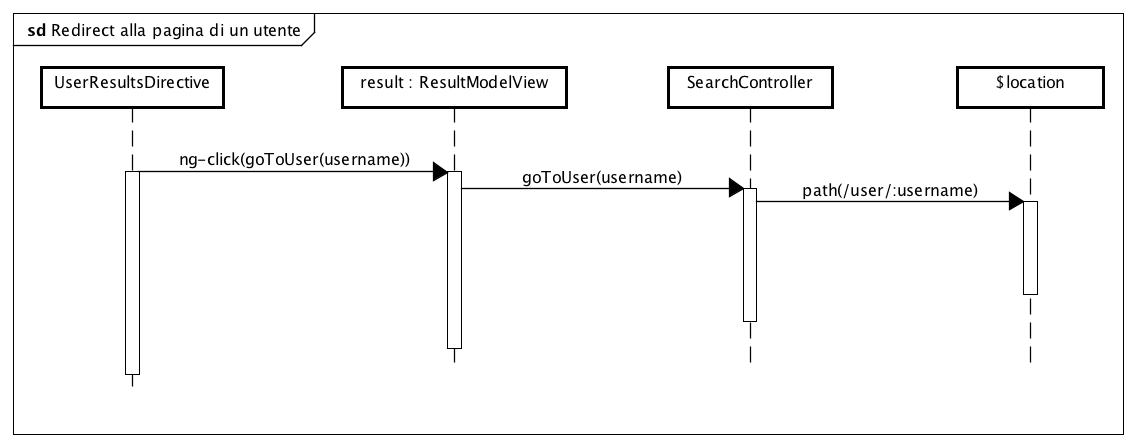
\includegraphics[scale=0.5,keepaspectratio]{UML/DiagrammiDiSequenza/Front-end/Search_goToUser.png}
	\caption{Redirect alla pagina di un utente}
\end{figure} \FloatBarrier

L'utente, posizionato dentro la pagina di ricerca, potrà decidere di visualizzare la pagina del profilo di altro utente azionando l'evento \texttt{ng-click} associato al bottone posizionato all'interno della \texttt{directive\ped{G}} \texttt{UserDetailDirective}.